\documentclass[conference]{IEEEtran}
% Floodline paper. Results are typeset only through the macros in numbers.tex and the tables in tables/, which
% paper/make_numbers.py writes from the result files; a result that does not exist yet renders as a grey
% "pending" marker. Do not type result numbers into this file.

\usepackage[T1]{fontenc}
\usepackage{cite}
\usepackage{amsmath,amssymb}
\usepackage{graphicx}
\usepackage{booktabs}
\usepackage{xcolor}
\usepackage{tikz}
\usetikzlibrary{positioning,arrows.meta}
\usepackage{array}
\usepackage[hidelinks]{hyperref}
\usepackage{url}

\newcommand{\pending}[1]{\textcolor{gray}{\textbf{[pending: #1]}}}
% Generated by paper/make_numbers.py from the result files; do not edit by hand.
% Each macro is followed by the file it was read from.
\newcommand{\nEvents}{6} % results/benchmark_summary.json
\newcommand{\nTowns}{11} % results/benchmark_summary.json
\newcommand{\nHexes}{10{,}886} % results/benchmark_summary.json
\newcommand{\nSevere}{3{,}806} % results/benchmark_summary.json
\newcommand{\nDraws}{1{,}000} % results/benchmark_summary.json
\newcommand{\blockRes}{6} % results/benchmark_summary.json
\newcommand{\wlImages}{538} % results/waterline_run.json
\newcommand{\capEHA}{0.76} % results/benchmark_summary.json
\newcommand{\capEHALo}{0.55} % results/benchmark_summary.json
\newcommand{\capEHAHi}{0.78} % results/benchmark_summary.json
\newcommand{\capEH}{0.78} % results/benchmark_summary.json
\newcommand{\capEHLo}{0.58} % results/benchmark_summary.json
\newcommand{\capEHHi}{0.80} % results/benchmark_summary.json
\newcommand{\dEH}{$-$0.016} % results/benchmark_summary.json
\newcommand{\dEHLo}{$-$0.071} % results/benchmark_summary.json
\newcommand{\dEHHi}{$+$0.005} % results/benchmark_summary.json
\newcommand{\pEH}{9\%} % results/benchmark_summary.json
\newcommand{\capEA}{0.66} % results/benchmark_summary.json
\newcommand{\capEALo}{0.55} % results/benchmark_summary.json
\newcommand{\capEAHi}{0.71} % results/benchmark_summary.json
\newcommand{\dEA}{$+$0.108} % results/benchmark_summary.json
\newcommand{\dEALo}{$-$0.068} % results/benchmark_summary.json
\newcommand{\dEAHi}{$+$0.135} % results/benchmark_summary.json
\newcommand{\pEA}{82\%} % results/benchmark_summary.json
\newcommand{\capHA}{0.64} % results/benchmark_summary.json
\newcommand{\capHALo}{0.47} % results/benchmark_summary.json
\newcommand{\capHAHi}{0.68} % results/benchmark_summary.json
\newcommand{\dHA}{$+$0.123} % results/benchmark_summary.json
\newcommand{\dHALo}{$+$0.019} % results/benchmark_summary.json
\newcommand{\dHAHi}{$+$0.210} % results/benchmark_summary.json
\newcommand{\pHA}{99\%} % results/benchmark_summary.json
\newcommand{\capRisk}{0.77} % results/benchmark_summary.json
\newcommand{\capRiskLo}{0.61} % results/benchmark_summary.json
\newcommand{\capRiskHi}{0.80} % results/benchmark_summary.json
\newcommand{\dRisk}{$-$0.005} % results/benchmark_summary.json
\newcommand{\dRiskLo}{$-$0.150} % results/benchmark_summary.json
\newcommand{\dRiskHi}{$+$0.044} % results/benchmark_summary.json
\newcommand{\pRisk}{30\%} % results/benchmark_summary.json
\newcommand{\capRiskA}{0.74} % results/benchmark_summary.json
\newcommand{\capRiskALo}{0.58} % results/benchmark_summary.json
\newcommand{\capRiskAHi}{0.78} % results/benchmark_summary.json
\newcommand{\dRiskA}{$+$0.027} % results/benchmark_summary.json
\newcommand{\dRiskALo}{$-$0.116} % results/benchmark_summary.json
\newcommand{\dRiskAHi}{$+$0.074} % results/benchmark_summary.json
\newcommand{\pRiskA}{53\%} % results/benchmark_summary.json
\newcommand{\capBuildings}{0.77} % results/benchmark_summary.json
\newcommand{\capBuildingsLo}{0.63} % results/benchmark_summary.json
\newcommand{\capBuildingsHi}{0.80} % results/benchmark_summary.json
\newcommand{\dBuildings}{$-$0.004} % results/benchmark_summary.json
\newcommand{\dBuildingsLo}{$-$0.166} % results/benchmark_summary.json
\newcommand{\dBuildingsHi}{$+$0.033} % results/benchmark_summary.json
\newcommand{\pBuildings}{23\%} % results/benchmark_summary.json
\newcommand{\capPeople}{0.70} % results/benchmark_summary.json
\newcommand{\capPeopleLo}{0.55} % results/benchmark_summary.json
\newcommand{\capPeopleHi}{0.76} % results/benchmark_summary.json
\newcommand{\dPeople}{$+$0.067} % results/benchmark_summary.json
\newcommand{\dPeopleLo}{$-$0.113} % results/benchmark_summary.json
\newcommand{\dPeopleHi}{$+$0.144} % results/benchmark_summary.json
\newcommand{\pPeople}{64\%} % results/benchmark_summary.json
\newcommand{\capE}{0.67} % results/benchmark_summary.json
\newcommand{\capELo}{0.57} % results/benchmark_summary.json
\newcommand{\capEHi}{0.73} % results/benchmark_summary.json
\newcommand{\dE}{$+$0.091} % results/benchmark_summary.json
\newcommand{\dELo}{$-$0.094} % results/benchmark_summary.json
\newcommand{\dEHi}{$+$0.117} % results/benchmark_summary.json
\newcommand{\pE}{72\%} % results/benchmark_summary.json
\newcommand{\capWater}{0.56} % results/benchmark_summary.json
\newcommand{\capWaterLo}{0.41} % results/benchmark_summary.json
\newcommand{\capWaterHi}{0.64} % results/benchmark_summary.json
\newcommand{\dWater}{$+$0.204} % results/benchmark_summary.json
\newcommand{\dWaterLo}{$+$0.020} % results/benchmark_summary.json
\newcommand{\dWaterHi}{$+$0.293} % results/benchmark_summary.json
\newcommand{\pWater}{99\%} % results/benchmark_summary.json
\newcommand{\capA}{0.33} % results/benchmark_summary.json
\newcommand{\capALo}{0.15} % results/benchmark_summary.json
\newcommand{\capAHi}{0.36} % results/benchmark_summary.json
\newcommand{\dA}{$+$0.435} % results/benchmark_summary.json
\newcommand{\dALo}{$+$0.278} % results/benchmark_summary.json
\newcommand{\dAHi}{$+$0.558} % results/benchmark_summary.json
\newcommand{\pA}{100\%} % results/benchmark_summary.json
\newcommand{\capPeopleEHA}{0.73} % results/benchmark_summary.json
\newcommand{\capPeopleEHALo}{0.51} % results/benchmark_summary.json
\newcommand{\capPeopleEHAHi}{0.74} % results/benchmark_summary.json
\newcommand{\dPeopleEHA}{$+$0.034} % results/benchmark_summary.json
\newcommand{\dPeopleEHALo}{$+$0.006} % results/benchmark_summary.json
\newcommand{\dPeopleEHAHi}{$+$0.119} % results/benchmark_summary.json
\newcommand{\pPeopleEHA}{100\%} % results/benchmark_summary.json
\newcommand{\meanEHA}{0.72} % results/benchmark_summary.json
\newcommand{\worstEHA}{0.37} % results/benchmark_summary.json
\newcommand{\worstEHAEvent}{Sanghar} % results/benchmark_summary.json
\newcommand{\meanEH}{0.73} % results/benchmark_summary.json
\newcommand{\worstEH}{0.40} % results/benchmark_summary.json
\newcommand{\worstEHEvent}{New South Wales} % results/benchmark_summary.json
\newcommand{\meanEA}{0.55} % results/benchmark_summary.json
\newcommand{\worstEA}{0.09} % results/benchmark_summary.json
\newcommand{\worstEAEvent}{Sanghar} % results/benchmark_summary.json
\newcommand{\meanHA}{0.61} % results/benchmark_summary.json
\newcommand{\worstHA}{0.19} % results/benchmark_summary.json
\newcommand{\worstHAEvent}{New South Wales} % results/benchmark_summary.json
\newcommand{\meanRisk}{0.68} % results/benchmark_summary.json
\newcommand{\worstRisk}{0.10} % results/benchmark_summary.json
\newcommand{\worstRiskEvent}{Moramanga} % results/benchmark_summary.json
\newcommand{\meanRiskA}{0.63} % results/benchmark_summary.json
\newcommand{\worstRiskA}{0.10} % results/benchmark_summary.json
\newcommand{\worstRiskAEvent}{Moramanga} % results/benchmark_summary.json
\newcommand{\meanBuildings}{0.67} % results/benchmark_summary.json
\newcommand{\worstBuildings}{0.07} % results/benchmark_summary.json
\newcommand{\worstBuildingsEvent}{Moramanga} % results/benchmark_summary.json
\newcommand{\meanPeople}{0.58} % results/benchmark_summary.json
\newcommand{\worstPeople}{0.22} % results/benchmark_summary.json
\newcommand{\worstPeopleEvent}{Sanghar} % results/benchmark_summary.json
\newcommand{\meanE}{0.57} % results/benchmark_summary.json
\newcommand{\worstE}{0.09} % results/benchmark_summary.json
\newcommand{\worstEEvent}{Sanghar} % results/benchmark_summary.json
\newcommand{\meanWater}{0.53} % results/benchmark_summary.json
\newcommand{\worstWater}{0.00} % results/benchmark_summary.json
\newcommand{\worstWaterEvent}{New South Wales} % results/benchmark_summary.json
\newcommand{\meanA}{0.28} % results/benchmark_summary.json
\newcommand{\worstA}{0.00} % results/benchmark_summary.json
\newcommand{\worstAEvent}{Sanghar} % results/benchmark_summary.json
\newcommand{\meanPeopleEHA}{0.69} % results/benchmark_summary.json
\newcommand{\worstPeopleEHA}{0.32} % results/benchmark_summary.json
\newcommand{\worstPeopleEHAEvent}{Sanghar} % results/benchmark_summary.json
\newcommand{\loeoDefault}{0.715} % results/benchmark_summary.json
\newcommand{\loeoFitted}{0.591} % results/benchmark_summary.json
\newcommand{\loeoBuildings}{0.672} % results/benchmark_summary.json
\newcommand{\loeoPeople}{0.578} % results/benchmark_summary.json
\newcommand{\loeoFittedMoramanga}{0.10} % results/benchmark_summary.json
\newcommand{\loeoFittedSanghar}{0.23} % results/benchmark_summary.json
\newcommand{\loeoAccessZero}{6 of 6} % results/benchmark_summary.json
\newcommand{\sensVariants}{131} % results/sensitivity_run.json
\newcommand{\sensPragueSpearmanMin}{0.98} % results/sensitivity_run.json
\newcommand{\sensPragueKeepEight}{86\%} % results/sensitivity_run.json
\newcommand{\roadAffPZero}{0.68} % results/benchmark_summary.json
\newcommand{\roadAffRZero}{0.80} % results/benchmark_summary.json
\newcommand{\roadAffFZero}{0.74} % results/benchmark_summary.json
\newcommand{\roadSevPZero}{0.26} % results/benchmark_summary.json
\newcommand{\roadSevRZero}{0.89} % results/benchmark_summary.json
\newcommand{\roadSevFZero}{0.40} % results/benchmark_summary.json
\newcommand{\roadAffPFive}{0.77} % results/benchmark_summary.json
\newcommand{\roadAffRFive}{0.77} % results/benchmark_summary.json
\newcommand{\roadAffFFive}{0.77} % results/benchmark_summary.json
\newcommand{\roadSevPFive}{0.29} % results/benchmark_summary.json
\newcommand{\roadSevRFive}{0.86} % results/benchmark_summary.json
\newcommand{\roadSevFFive}{0.44} % results/benchmark_summary.json
\newcommand{\roadAffPFifteen}{0.78} % results/benchmark_summary.json
\newcommand{\roadAffRFifteen}{0.70} % results/benchmark_summary.json
\newcommand{\roadAffFFifteen}{0.74} % results/benchmark_summary.json
\newcommand{\roadSevPFifteen}{0.29} % results/benchmark_summary.json
\newcommand{\roadSevRFifteen}{0.76} % results/benchmark_summary.json
\newcommand{\roadSevFFifteen}{0.42} % results/benchmark_summary.json
\newcommand{\roadAffPFifty}{0.79} % results/benchmark_summary.json
\newcommand{\roadAffRFifty}{0.48} % results/benchmark_summary.json
\newcommand{\roadAffFFifty}{0.60} % results/benchmark_summary.json
\newcommand{\roadSevPFifty}{0.28} % results/benchmark_summary.json
\newcommand{\roadSevRFifty}{0.50} % results/benchmark_summary.json
\newcommand{\roadSevFFifty}{0.36} % results/benchmark_summary.json
\newcommand{\ablChangeEHA}{\pending{sentinel1\_change: EHA}} % results/benchmark_summary.json -- missing: sentinel1_change: 6 of 11 towns so far
\newcommand{\ablChangeEHARef}{\pending{sentinel1\_change: reference EHA}} % results/benchmark_summary.json -- missing: sentinel1_change: 6 of 11 towns so far
\newcommand{\ablChangeBuildings}{\pending{sentinel1\_change: buildings\_in\_flood}} % results/benchmark_summary.json -- missing: sentinel1_change: 6 of 11 towns so far
\newcommand{\ablChangeBuildingsRef}{\pending{sentinel1\_change: reference buildings\_in\_flood}} % results/benchmark_summary.json -- missing: sentinel1_change: 6 of 11 towns so far
\newcommand{\ablChangeWater}{\pending{sentinel1\_change: water}} % results/benchmark_summary.json -- missing: sentinel1_change: 6 of 11 towns so far
\newcommand{\ablChangeWaterRef}{\pending{sentinel1\_change: reference water}} % results/benchmark_summary.json -- missing: sentinel1_change: 6 of 11 towns so far
\newcommand{\ablOtsuEHA}{\pending{sentinel1\_otsu: EHA}} % results/benchmark_summary.json -- missing: key data_ablations/sentinel1_otsu
\newcommand{\ablOtsuEHARef}{\pending{sentinel1\_otsu: reference EHA}} % results/benchmark_summary.json -- missing: key data_ablations/sentinel1_otsu
\newcommand{\ablOtsuBuildings}{\pending{sentinel1\_otsu: buildings\_in\_flood}} % results/benchmark_summary.json -- missing: key data_ablations/sentinel1_otsu
\newcommand{\ablOtsuBuildingsRef}{\pending{sentinel1\_otsu: reference buildings\_in\_flood}} % results/benchmark_summary.json -- missing: key data_ablations/sentinel1_otsu
\newcommand{\ablOtsuWater}{\pending{sentinel1\_otsu: water}} % results/benchmark_summary.json -- missing: key data_ablations/sentinel1_otsu
\newcommand{\ablOtsuWaterRef}{\pending{sentinel1\_otsu: reference water}} % results/benchmark_summary.json -- missing: key data_ablations/sentinel1_otsu
\newcommand{\ablOSMOnlyEHA}{\pending{osm\_only: EHA}} % results/benchmark_summary.json -- missing: key data_ablations/osm_only
\newcommand{\ablOSMOnlyEHARef}{\pending{osm\_only: reference EHA}} % results/benchmark_summary.json -- missing: key data_ablations/osm_only
\newcommand{\ablOSMOnlyBuildings}{\pending{osm\_only: buildings\_in\_flood}} % results/benchmark_summary.json -- missing: key data_ablations/osm_only
\newcommand{\ablOSMOnlyBuildingsRef}{\pending{osm\_only: reference buildings\_in\_flood}} % results/benchmark_summary.json -- missing: key data_ablations/osm_only
\newcommand{\ablOSMOnlyWater}{\pending{osm\_only: water}} % results/benchmark_summary.json -- missing: key data_ablations/osm_only
\newcommand{\ablOSMOnlyWaterRef}{\pending{osm\_only: reference water}} % results/benchmark_summary.json -- missing: key data_ablations/osm_only
\newcommand{\radarErftstadtShare}{0.5\%} % results/benchmark_s1/EMSR517/event_run.json
\newcommand{\radarErftstadtScene}{2021-07-18} % results/benchmark_s1/EMSR517/event_run.json
\newcommand{\radarErftstadtPre}{2021-07-06} % results/benchmark_s1/EMSR517/event_run.json
\newcommand{\emsErftstadtShare}{20.9\%} % results/benchmark/EMSR517/satellite_run_aoi07.json
\newcommand{\radarSangharShare}{0.8\%} % results/benchmark_s1/EMSR631/event_run.json
\newcommand{\radarSangharScene}{2022-09-11} % results/benchmark_s1/EMSR631/event_run.json
\newcommand{\radarSangharPre}{2022-08-30} % results/benchmark_s1/EMSR631/event_run.json
\newcommand{\emsSangharShare}{72.8\%} % results/benchmark/EMSR631/satellite_run_aoi01.json
\newcommand{\trustRefs}{11{,}563} % results/trust_eval.json
\newcommand{\trustSample}{500} % results/trust_eval.json
\newcommand{\trustForwarded}{99.8\%} % results/trust_eval.json
\newcommand{\trustCropped}{21.8\%} % results/trust_eval.json
\newcommand{\trustBandN}{27} % results/trust_eval.json
\newcommand{\trustEufloodN}{3{,}710} % results/trust_eval.json
\newcommand{\trustBandShare}{0.7\%} % results/trust_eval.json
\newcommand{\trustRejectBits}{2} % results/trust_eval.json
\newcommand{\leakEuflood}{2{,}371} % results/trust_eval.json
\newcommand{\leakTest}{20} % results/trust_eval.json
\newcommand{\leakTestN}{1{,}180} % results/trust_eval.json
\newcommand{\atkLoneOverlap}{1.00} % results/attack_prague.json
\newcommand{\atkLoneFlagged}{50/50} % results/attack_prague.json
\newcommand{\atkLoneInTop}{0} % results/attack_prague.json
\newcommand{\atkColludeOverlap}{1.00} % results/attack_prague.json
\newcommand{\atkColludeFlagged}{10/10} % results/attack_prague.json
\newcommand{\atkColludeInTop}{0} % results/attack_prague.json
\newcommand{\atkWetOverlap}{0.91} % results/attack_prague.json
\newcommand{\atkWetFlagged}{50/50} % results/attack_prague.json
\newcommand{\atkWetInTop}{3.2} % results/attack_prague.json
\newcommand{\permLoneOverlap}{1.00} % results/attack_prague_permissive.json
\newcommand{\permLoneFlagged}{50/50} % results/attack_prague_permissive.json
\newcommand{\permLoneInTop}{0} % results/attack_prague_permissive.json
\newcommand{\permColludeOverlap}{0.30} % results/attack_prague_permissive.json
\newcommand{\permColludeFlagged}{0/10} % results/attack_prague_permissive.json
\newcommand{\permColludeInTop}{7} % results/attack_prague_permissive.json
\newcommand{\permWetOverlap}{0.39} % results/attack_prague_permissive.json
\newcommand{\permWetFlagged}{0/50} % results/attack_prague_permissive.json
\newcommand{\permWetInTop}{8.35} % results/attack_prague_permissive.json
\newcommand{\atkDraws}{20} % results/attack_prague.json
\newcommand{\samImages}{538} % results/sam3_run.json
\newcommand{\samCalls}{686} % results/sam3_run.json
\newcommand{\samWaterMean}{0.959} % results/sam3_run.json
\newcommand{\samWaterMedian}{0.989} % results/sam3_run.json
\newcommand{\samWaterN}{482} % results/sam3_run.json
\newcommand{\samPersonMean}{0.882} % results/sam3_run.json
\newcommand{\samPersonMedian}{0.945} % results/sam3_run.json
\newcommand{\samPersonN}{138} % results/sam3_run.json
\newcommand{\samBuildingMean}{0.775} % results/sam3_run.json
\newcommand{\samBuildingMedian}{0.948} % results/sam3_run.json
\newcommand{\samBuildingN}{229} % results/sam3_run.json
\newcommand{\samWaterBF}{0.960} % results/sam3_run.json
\newcommand{\wlWithEstimate}{135} % results/waterline_run.json
\newcommand{\wlN}{40} % results/waterline_run.json
\newcommand{\wlExact}{0.40} % results/waterline_run.json
\newcommand{\wlWithin}{0.78} % results/waterline_run.json
\newcommand{\wlMAE}{0.85} % results/waterline_run.json
\newcommand{\wlBaseExact}{0.38} % results/waterline_depth.csv + data/depth_labels.csv
\newcommand{\wlBaseWithin}{0.83} % results/waterline_depth.csv + data/depth_labels.csv
\newcommand{\wlDryRight}{10 of 11} % results/waterline_depth.csv + data/depth_labels.csv
\newcommand{\wlAnkleKnee}{7 of 15} % results/waterline_depth.csv + data/depth_labels.csv
\newcommand{\wlAboveHeadN}{0} % results/waterline_depth.csv + data/depth_labels.csv
\newcommand{\vlmN}{\pending{VLM benchmark images}} % results/vlm_benchmark.json -- missing: results/vlm_benchmark.json: run in progress (49 images assessed)
\newcommand{\vlmExact}{\pending{two-pass Qwen3-VL-8B exact class accuracy}} % results/vlm_benchmark.json -- missing: results/vlm_benchmark.json: run in progress (49 images assessed)
\newcommand{\vlmWithin}{\pending{two-pass Qwen3-VL-8B within-one accuracy}} % results/vlm_benchmark.json -- missing: results/vlm_benchmark.json: run in progress (49 images assessed)
\newcommand{\vlmBaseExact}{\pending{majority baseline on the VLM-assessed images}} % results/vlm_benchmark.json -- missing: results/vlm_benchmark.json: run in progress (49 images assessed)
\newcommand{\depthImages}{300} % results/release_run.json
\newcommand{\depthUnknown}{203} % results/release_run.json
\newcommand{\eufRecords}{3{,}435} % results/external_run.json
\newcommand{\eufLocated}{883} % results/external_run.json
\newcommand{\agInAoi}{442} % results/agreement_euflood_run.json
\newcommand{\agOwnHex}{50.2\%} % results/agreement_euflood_run.json
\newcommand{\agRing}{56.6\%} % results/agreement_euflood_run.json
\newcommand{\agRingPerm}{100\%} % results/agreement_euflood_run.json
\newcommand{\agDresdenN}{171} % results/agreement_euflood_run.json
\newcommand{\agDresdenFlood}{142} % results/agreement_euflood_run.json
\newcommand{\agDresdenRiver}{35} % results/agreement_euflood_run.json
\newcommand{\agDresdenNear}{92.4\%} % results/agreement_euflood_run.json
\newcommand{\agPragueN}{252} % results/agreement_euflood_run.json
\newcommand{\agPragueFlood}{3{,}102} % results/agreement_euflood_run.json
\newcommand{\agPragueRiver}{21} % results/agreement_euflood_run.json
\newcommand{\agPragueNear}{87.7\%} % results/agreement_euflood_run.json
\newcommand{\pragueClosed}{39} % results/reach_prague_run.json
\newcommand{\pragueUnderWater}{4.22} % results/reach_prague_run.json
\newcommand{\pragueCut}{10} % results/reach_prague_run.json
\newcommand{\pragueBuildings}{116} % results/exposure_prague_run.json
\newcommand{\pragueTopBuildings}{45} % results/hexes_prague_run.json
\newcommand{\praguePhotos}{203} % docs/map/cities.json
\newcommand{\larkClosed}{2{,}320} % results/reach_larkana_run.json
\newcommand{\larkUnderWater}{365} % results/reach_larkana_run.json
\newcommand{\larkCut}{678} % results/reach_larkana_run.json
\newcommand{\larkOSM}{108} % results/exposure_larkana_run.json
\newcommand{\larkMS}{78{,}848} % results/exposure_larkana_run.json
\newcommand{\larkHexes}{7{,}663} % results/exposure_larkana_run.json
\newcommand{\larkBuildingsFlood}{10{,}175} % docs/map/cities.json
\newcommand{\sOneIoU}{0.74} % results/sentinel1_larkana_run.json
\newcommand{\sOneP}{0.94} % results/sentinel1_larkana_run.json
\newcommand{\sOneR}{0.78} % results/sentinel1_larkana_run.json
\newcommand{\sOneShareRadar}{0.48} % results/sentinel1_larkana_run.json
\newcommand{\sOneShareEMS}{0.59} % results/sentinel1_larkana_run.json
\newcommand{\sOneSpearman}{0.94} % results/sentinel1_larkana_run.json
\newcommand{\sOneHexes}{8{,}337} % results/sentinel1_larkana_run.json
\newcommand{\sOneThreshold}{-12.9} % results/sentinel1_larkana_run.json

\newcommand{\ci}[2]{[#1,\,#2]}

\begin{document}

\title{Floodline: Ranking Where Flood Responders Are Needed}

\author{\IEEEauthorblockN{Sunny Shaban Ali}
\IEEEauthorblockA{Department of Computer Science\\
National University of Computer and Emerging Sciences (FAST-NUCES)\\
Karachi, Pakistan\\
reach@sunnyshabanali.dev}}

\maketitle

\begin{abstract}
A district flood coordinator has to decide where boats and relief go first. Floodline ranks H3 hexagons by fusing three layers anyone can obtain within a day of a flood: the Copernicus Emergency Management Service (EMS) flood extent, the buildings inside it, and road access from fire stations and hospitals with flooded roads removed. We test the ranking against analysts' damage grades on every town with at least 20 damaged or destroyed buildings in six EMS activations: Germany 2021, Pakistan 2022, Australia 2021, Madagascar 2022 and two in Italy (\nTowns{} towns, \nHexes{} hexagons, \nSevere{} graded buildings). The top 10\% of hexagons by fused priority contain \capEHA{} of each town's damage on average (95\% spatial block-bootstrap interval \ci{\capEHALo}{\capEHAHi}; random 0.10). That is level with counting buildings in the flood and \dWater{} against flood extent alone. What separates the scores is the worst case: every building, water, exposure or access layer alone falls to 0.10 or below on at least one flood, while the fused priority's worst event is \worstEHA{}. Weights fitted on five floods and tested on the sixth do worse than the hand-set default (\loeoFitted{} against \loeoDefault{} held-out mean). Access does not change damage capture; it stays because reachability is the other half of a coordinator's question. Replacing the analysts' map with Sentinel-1 radar drops capture to \ablChangeEHA{} (change detection) or \ablOtsuEHA{} (thresholding), so radar alone does not yet support ranking within towns; OpenStreetMap-only buildings cost little pooled but cut capture where OSM is thin (New South Wales \osmOnlyNSWRef{} to \osmOnlyNSW{}, Sanghar \osmOnlySangharRef{} to \osmOnlySanghar{}). A report trust model keeps simulated colluding devices out of the top ten. We release the pipeline, the benchmark, a web map, an offline field app and a flood-depth benchmark, and report the negative results.
\end{abstract}

\begin{IEEEkeywords}
flood response, rapid mapping, Copernicus EMS, damage grading, network accessibility, H3, benchmark
\end{IEEEkeywords}

% ===============================================================================================================
\section{Introduction}

Rapid-mapping services publish flood extent polygons within hours to days of an activation~\cite{cems_rapid,donezar2020validation}. A coordinator still has to turn a flood map into an order of work: which neighbourhoods first, and which of those a ground team can still reach. Ground photos help where they exist, but people surrounded by water rarely take them, so the hexagons that most need help tend to have the fewest~\cite{assumpcao2018citizen}.

Floodline scores every hexagon inside the mapped area from three layers: hazard (the share of the hexagon under water), exposure (buildings in the water, or in a hexagon the flood cuts off) and access (cut off from the road network, or forced into a detour). Photos and field reports refine the score only when something independent corroborates them.

A ranking is only useful if it is right on floods it was not tuned on. We therefore evaluate against EMS damage grading, which analysts produce from post-event imagery without our layers, on six activations chosen by a fixed rule, and ask five questions:
\begin{itemize}
\item \textbf{RQ1} Does the fused priority find damage across floods and continents?
\item \textbf{RQ2} Which components matter?
\item \textbf{RQ3} Is it robust to a flood it has not seen?
\item \textbf{RQ4} What changes with radar instead of analysts' maps, or OpenStreetMap-only buildings?
\item \textbf{RQ5} Can reports from the field be trusted under attack?
\end{itemize}

Our contributions are a multi-event benchmark protocol for responder rankings with spatial block-bootstrap intervals and leave-one-event-out validation (Sec.~\ref{sec:bench}); the finding that a hand-set fused score has the best held-out mean and a far better worst case than any single layer, while fitted weights overfit (Sec.~\ref{sec:rq3}); a flood-aware road closure rule validated against graded road damage; a report trust model tested by simulated collusion (Sec.~\ref{sec:trust}); and an open pipeline, map, field app and depth benchmark, with negative results stated.

% ===============================================================================================================
\section{Related Work}

\textbf{Satellite flood mapping.} The Copernicus EMS rapid-mapping component produces flood delineation and damage-grading products on activation~\cite{cems_rapid}; its validation service studies Sentinel-1 backscatter and coherence for flood monitoring~\cite{donezar2020validation}. Sen1Floods11 provides labelled Sentinel-1 chips for flood segmentation~\cite{bonafilia2020sen1floods11}, and foundation models such as Prithvi-EO-2.0 are fine-tuned for it~\cite{szwarcman2024prithvi}.

\textbf{Citizen observations and photos.} Fohringer et al.\ derived inundation extent and depth from eyewitness photos of the 2013 Dresden flood~\cite{fohringer2015social}; Assump\c{c}\~ao et al.\ review citizen data across the flood modelling cycle~\cite{assumpcao2018citizen}. MediaEval 2017 combined social-media image retrieval with satellite flood segmentation~\cite{bischke2017mediaeval}, and Barz et al.\ released the European Flood 2013 photo set with expert relevance labels~\cite{barz2018flood}. Depth has been estimated from the submerged fraction of objects of known size~\cite{chaudhary2019water} and with fine-tuned vision--language models~\cite{fuad2026floodllama}.

\textbf{Accessibility under flooding.} Green et al.\ modelled emergency-responder access in Leicester under modelled flood scenarios~\cite{green2017accessibility}, and Pregnolato et al.\ fitted a depth--disruption function for vehicle speed~\cite{pregnolato2017depth}. We apply the idea to observed rapid-mapping polygons and OpenStreetMap~\cite{haklay2008osm} networks built with OSMnx~\cite{boeing2017osmnx}, and validate closures against graded road damage. We know of no prior evaluation of a responder ranking against damage grading across several events with held-out validation.

% ===============================================================================================================
\section{System}\label{sec:method}

\begin{figure}[t]
\centering
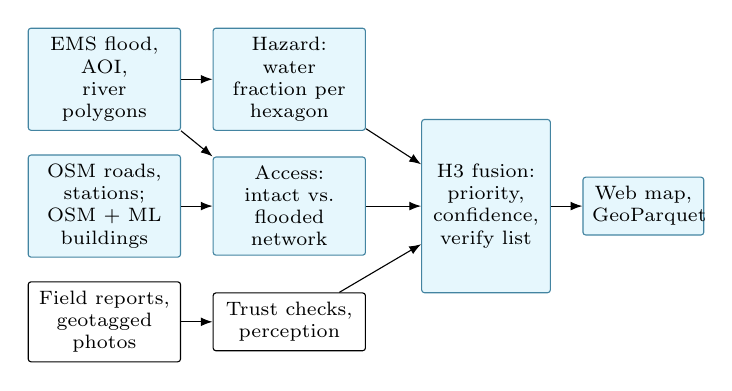
\begin{tikzpicture}[node distance=3mm and 4mm, font=\scriptsize,
  box/.style={draw, rounded corners=1pt, align=center, minimum height=6mm, text width=17mm},
  geo/.style={box, fill=cyan!10, draw=cyan!60!black},
  arr/.style={-{Latex[length=1.5mm]}}]
\node[geo] (ems) {EMS flood, AOI,\\river polygons};
\node[geo, below=of ems] (osm) {OSM roads, stations;\\OSM + ML buildings};
\node[box, below=of osm] (photo) {Field reports,\\geotagged photos};
\node[geo, right=of ems] (sat) {Hazard: water\\fraction per hexagon};
\node[geo, right=of osm] (reach) {Access: intact vs.\\flooded network};
\node[box, right=of photo] (perc) {Trust checks,\\perception};
\node[geo, right=7mm of reach, text width=14mm, minimum height=22mm] (fuse) {H3 fusion:\\priority,\\confidence,\\verify list};
\node[geo, right=of fuse, text width=13mm] (map) {Web map,\\GeoParquet};
\draw[arr] (ems) -- (sat); \draw[arr] (osm) -- (reach); \draw[arr] (ems.south east) -- (reach.north west);
\draw[arr] (photo) -- (perc); \draw[arr] (sat) -- (fuse); \draw[arr] (reach) -- (fuse); \draw[arr] (perc) -- (fuse);
\draw[arr] (fuse) -- (map);
\end{tikzpicture}
\caption{Floodline data flow. Shaded boxes are geospatial layers available within a day of an activation.}
\label{fig:system}
\end{figure}

Fig.~\ref{fig:system} shows the data flow. Every stage writes a run manifest with the code version, parameters and timing next to its output, and every number in this paper is read from those files by a script.

\textbf{Hazard.} For each EMS package we read the flood extent, the area of interest (AOI) and permanent water. Inside the AOI and outside the flood is a real zero; outside every AOI is unknown, never dry. Hazard $H$ is the hexagon's share inside the flood polygons; permanent water is kept apart, because a photo of a high river is not a photo of a flooded street (Sec.~\ref{sec:cases}). Towns use H3 resolution 9 (about 0.1\,km$^2$)~\cite{h3}.

\textbf{Access.} We take the OSM drive network for the AOI buffered by 1.5\,km, impute speeds by road class, and use fire stations and hospitals outside the flood as sources; if none lies near, the search widens to 15\,km. A station that does not snap to the downloaded network enters through a virtual source joined to its nearest road node, the gap costed at 30\,km/h. Multi-source Dijkstra~\cite{dijkstra1959note} gives travel time on the intact network; we remove every road with at least 5\,m inside the flood polygons and route again. A hexagon is \emph{cut off} if it has a road, is reachable intact and unreachable flooded; otherwise the detour $\Delta t$ is the difference. Access is $A=\max(c,\min(1,\Delta t/30\,\mathrm{min}))$ with $c=1$ for cut off.

\textbf{Exposure.} We count building footprints intersecting the flood ($B_\mathrm{f}$) and in total ($B$), taking per hexagon the larger of the OpenStreetMap and Microsoft Global ML Building Footprints~\cite{msbuildings} counts, which fills coverage gaps without double counting. Then $E=1-\exp(-(B_\mathrm{f}+c\,(B-B_\mathrm{f})+5P)/20)$, where $P$ counts corroborated people in water or stranded. A population variant uses GHSL 2020~\cite{ghsl2023pop}.

\textbf{Priority.} $\text{priority}=\mathbf{1}[H>0\lor c]\,(0.45E+0.30H+0.25A)$: zero unless the hexagon is wet or cut off. The weights are a prior set before any evaluation. Confidence is reported separately, from the number of independent layers and corroborating photos, so a high priority with low confidence is a hexagon to verify first.

\textbf{Field capture.} The Floodline Field web app captures a photo with time, location and quick tags (people, depth band, note), queues reports offline in IndexedDB, and uploads when there is signal. Location comes from EXIF GPS first, otherwise from the phone's fix only if the photo is under 10 minutes old, otherwise none. Reports enter the score only through the trust rules of Sec.~\ref{sec:trust} (Fig.~\ref{fig:app}).

\begin{figure}[t]
\centering
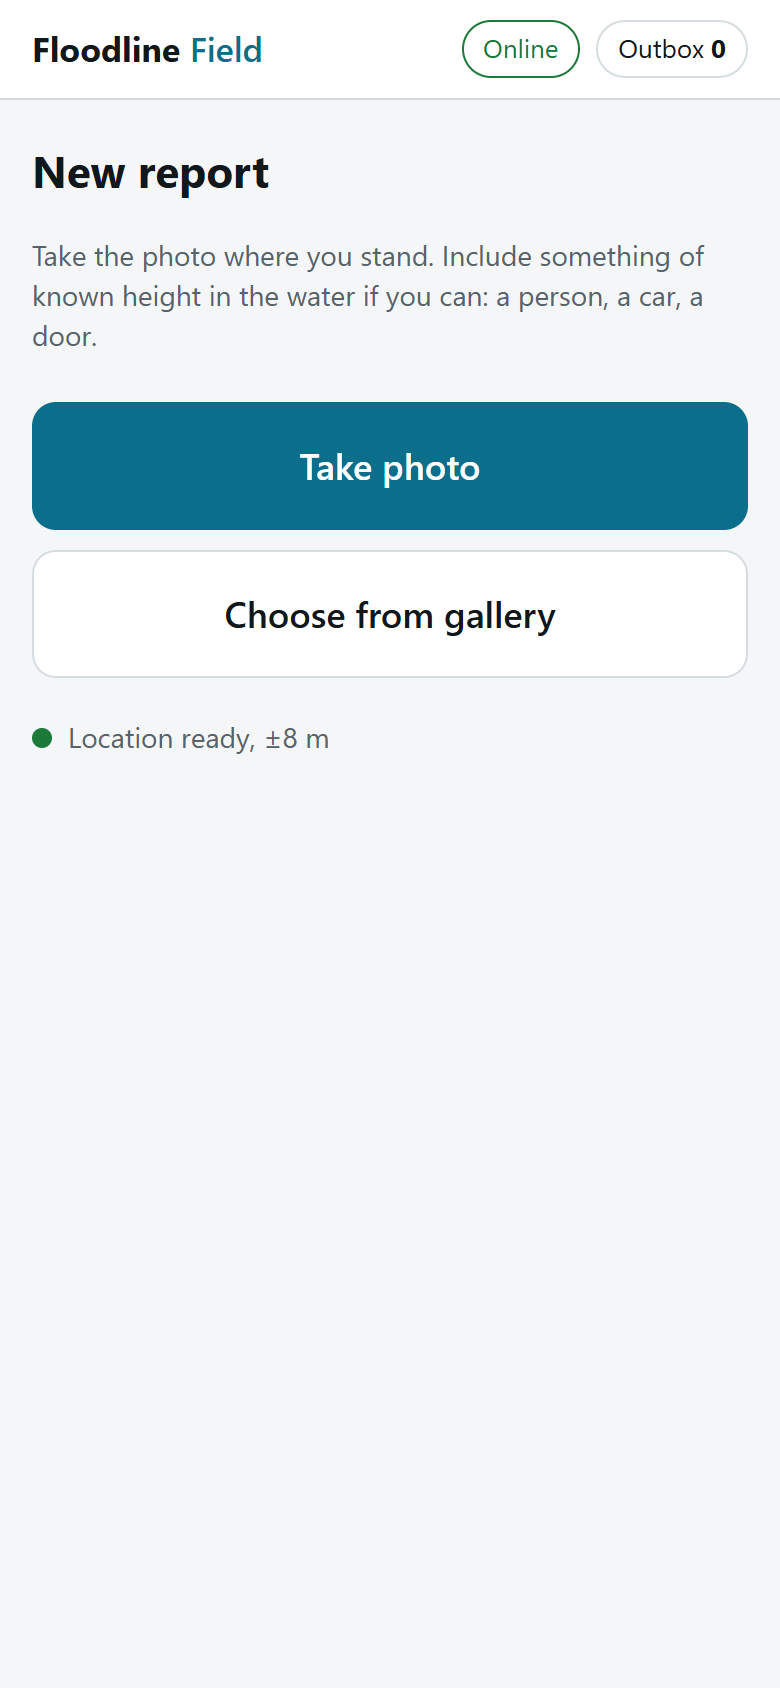
\includegraphics[width=0.31\columnwidth]{figures/app_capture.png}\hfill
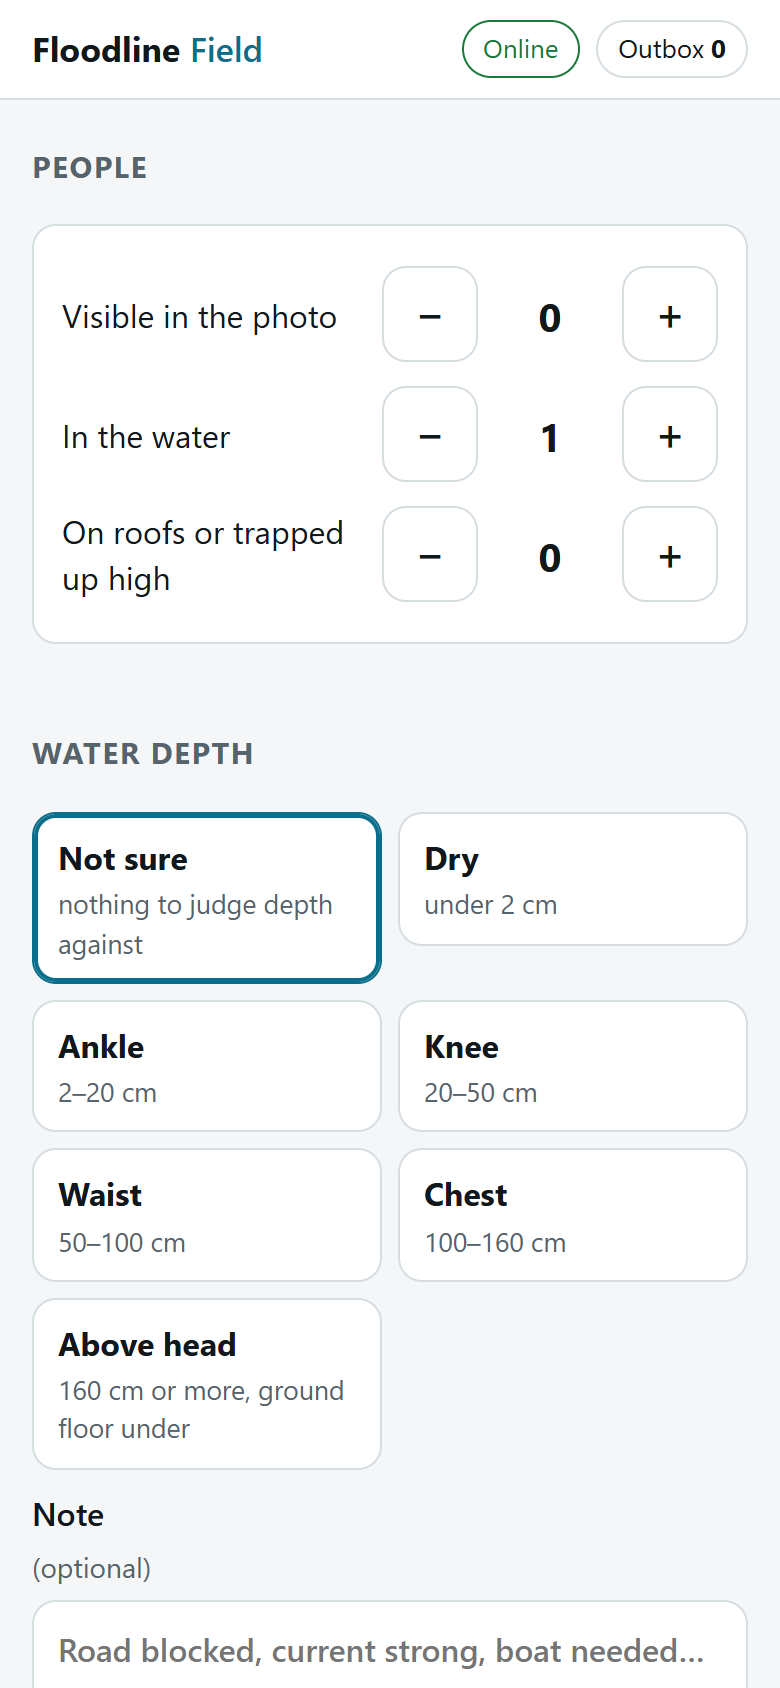
\includegraphics[width=0.31\columnwidth]{figures/app_details.png}\hfill
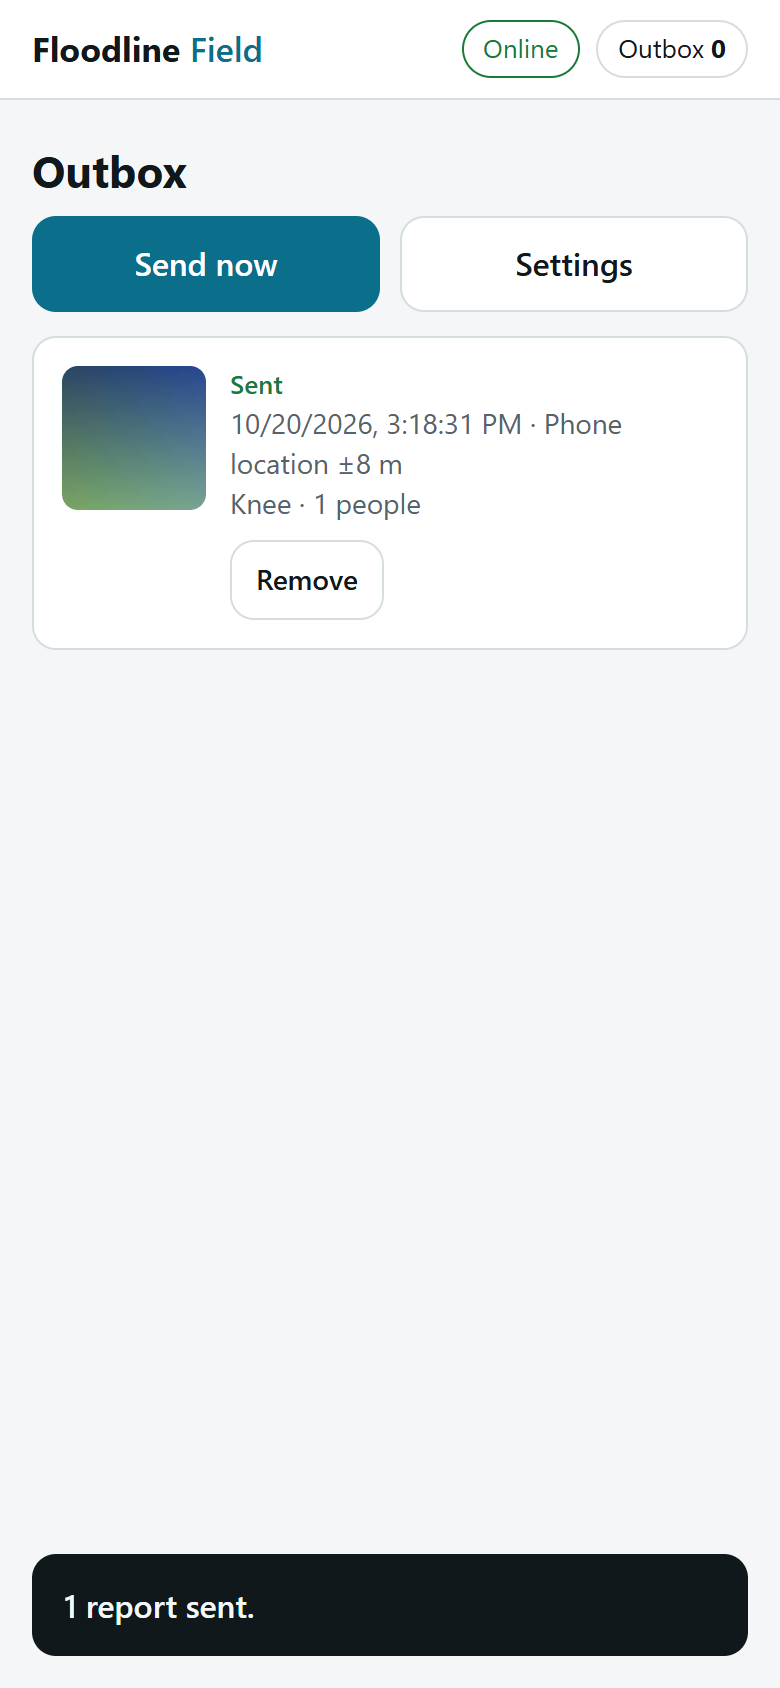
\includegraphics[width=0.31\columnwidth]{figures/app_outbox.png}
\caption{Floodline Field: capture with a live location fix, people and depth tags, and the outbox that holds reports until there is signal.}
\label{fig:app}
\end{figure}

% ===============================================================================================================
\section{Benchmark and Protocol}\label{sec:bench}

\textbf{Selection.} We take every EMS activation with damage-grading products and, within it, every town with at least 20 buildings graded damaged or destroyed (Table~\ref{tab:events}). The rule fixes the sample before any score is computed. OSM comes from Geofabrik extracts pinned by date.

\begin{table*}[t]
\caption{The benchmark: every town with at least 20 damaged or destroyed buildings in six EMS grading activations.}
\label{tab:events}
\centering\footnotesize
% Generated by make_numbers.py from docs/site.json and results/benchmark_towns.csv
\setlength{\tabcolsep}{4pt}
\begin{tabular}{@{}llllp{45mm}rr@{}}
\toprule
Activation & Area & Date & Type & Towns & Hexagons & Damaged or destroyed \\
\midrule
EMSR517 & Western Germany & July 2021 & flash flood & Erftstadt, Eschweiler, Wassenberg, Bad Neuenahr-Ahrweiler & 2{,}872 & 1{,}143 \\
EMSR631 & Sanghar, Sindh, Pakistan & September 2022 & riverine flood & Sanghar & 237 & 2{,}008 \\
EMSR504 & New South Wales, Australia & March 2021 & riverine flood & Kempsey & 808 & 78 \\
EMSR559 & Moramanga, Madagascar & January 2022 & flood & Moramanga & 1{,}568 & 69 \\
EMSR634 & Marche, Italy & September 2022 & flash flood & Cantiano, Ostra, Senigallia & 2{,}884 & 474 \\
EMSR649 & Pachino, Sicily, Italy & February 2023 & flash flood & Pachino & 2{,}517 & 34 \\
\midrule
Total & & & & 11 towns & 10{,}886 & 3{,}806 \\
\bottomrule
\end{tabular}

\end{table*}

\textbf{Metric.} For each town, the share of its damaged or destroyed buildings inside its top 10\% of hexagons by a score; the reported number is the mean over towns (random scores 0.10). ``Possibly damaged'' is excluded as a target because it follows the flood extent almost mechanically and would reward any extent-based score.

\textbf{Uncertainty.} Hexagons are spatially correlated, so we use a spatial block bootstrap~\cite{kunsch1989jackknife}: H3 resolution-\blockRes{} blocks resampled within towns, \nDraws{} draws. Differences are paired on the same draws.

\textbf{Variants.} Single layers: water extent ($H$), buildings in the flood ($B_\mathrm{f}$), people in the flood (GHSL), exposure ($E$) and access ($A$) alone. Fused: the default $EHA$; $EH$, $EA$, $HA$ keeping the default weights' proportions; and the risk form $E\,(0.5+0.5H)$.

\textbf{Held-out validation.} Leave one event out: the scoring rule (additive weights on a 0.05 simplex, or the risk form with an access weight; buildings or people as exposure) is fitted on five events and scored on the sixth.

% ===============================================================================================================
\section{Results}\label{sec:results}

\subsection{RQ1: Does the fused priority find damage?}
Fig.~\ref{fig:pooled} shows mean top-10\% capture over the \nTowns{} towns. The default fused priority captures \capEHA{} \ci{\capEHALo}{\capEHAHi}. Paired differences, default minus the other score: flood extent alone \dWater{} \ci{\dWaterLo}{\dWaterHi}, an interval that excludes zero; buildings in the flood \dBuildings{} \ci{\dBuildingsLo}{\dBuildingsHi}; people in the flood \dPeople{} \ci{\dPeopleLo}{\dPeopleHi}. Pooled, the fused priority is clearly better than the flood map alone and level with the best single exposure layer.

\begin{figure}[t]
\centering
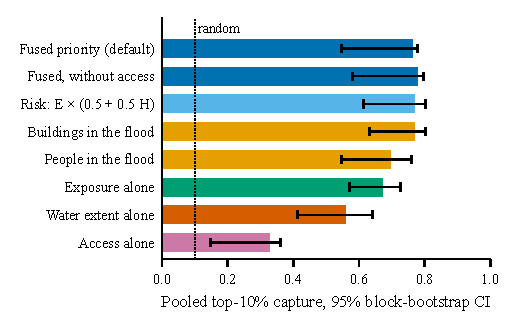
\includegraphics[width=\columnwidth]{figures/fig_pooled.pdf}
\caption{Mean top-10\% capture of damaged or destroyed buildings over \nTowns{} towns, with 95\% spatial block-bootstrap intervals.}
\label{fig:pooled}
\end{figure}

\subsection{RQ2: Which components matter?}
Default minus the no-access variant is \dEH{} \ci{\dEHLo}{\dEHHi}: access is neutral for damage capture, and the interval includes zero. Access alone captures \capA{}, so it carries little damage signal by itself. We keep it in the score for a reason damage grading cannot measure: a coordinator also needs to know which damaged places a ground team can reach, and closed roads and cut-off hexagons are drawn as their own layer. Default minus the variant without hazard ($EA$) is \dEA{} \ci{\dEALo}{\dEAHi}, and minus the variant without exposure ($HA$) \dHA{} \ci{\dHALo}{\dHAHi}: exposure is the term the score cannot lose. Default minus the same score with GHSL population as exposure is \dPeopleEHA{} \ci{\dPeopleEHALo}{\dPeopleEHAHi}.

\textbf{Road closures.} Against EMS road grading in the same towns, the closure rule's precision rises and recall falls with the overlap required (Fig.~\ref{fig:roads}). At 5\,m, precision is \roadAffPFive{} and recall \roadAffRFive{} against roads graded with any damage (F1 \roadAffFFive{}, against \roadAffFZero{} at 0\,m and \roadAffFFifteen{} at 15\,m). Against damaged or destroyed roads only, recall at 5\,m is \roadSevRFive{} and precision \roadSevPFive{}: most roads under water were impassable without visible damage, which a closure rule should capture.

\begin{figure}[t]
\centering
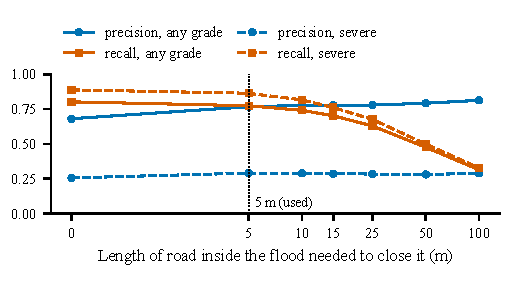
\includegraphics[width=\columnwidth]{figures/fig_roads.pdf}
\caption{Closure rule against EMS road grading for overlap thresholds of 0--100\,m; ``severe'' is damaged or destroyed.}
\label{fig:roads}
\end{figure}

\subsection{RQ3: Is it robust?}\label{sec:rq3}
Fig.~\ref{fig:events} breaks capture down by event. Every building, water, exposure or access layer collapses on at least one flood: buildings in the flood to \worstBuildings{} in \worstBuildingsEvent{}, where the footprints under the water are not where the damage was graded; water extent to \worstWater{} in \worstWaterEvent{}, where the whole plain is wet; exposure alone to \worstE{} and access alone to \worstA{} in \worstAEvent{}. The risk form inherits the buildings layer's failure (\worstRisk{} in \worstRiskEvent{}). Population alone bottoms at \worstPeople{} (\worstPeopleEvent{}). The fused scores do not collapse: the default's worst event is \worstEHA{} (\worstEHAEvent{}) and the no-access variant's \worstEH{}.

\begin{figure*}[t]
\centering
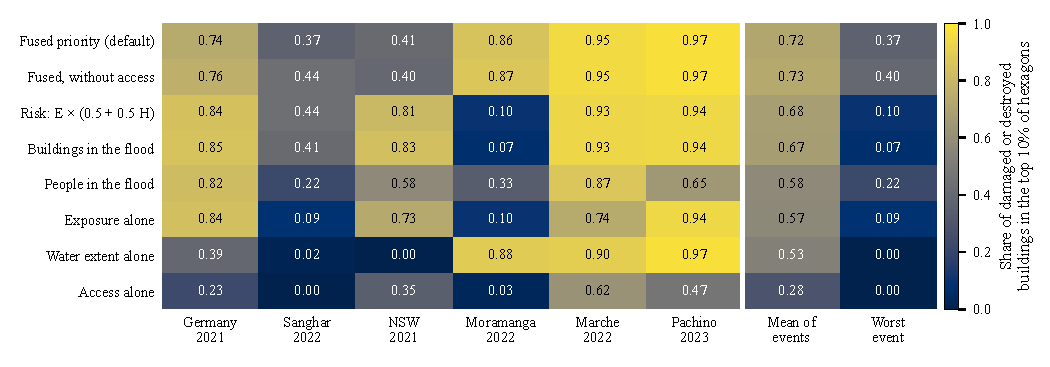
\includegraphics[width=\textwidth]{figures/fig_events.pdf}
\caption{Top-10\% capture of damaged or destroyed buildings per event (mean over its towns), with the mean and the worst event per score.}
\label{fig:events}
\end{figure*}

Table~\ref{tab:loeo} fits the scoring rule on five events and scores the sixth. The fitted rule has the lowest held-out mean of the fused and building scores (\loeoFitted{}), against \loeoDefault{} for the default and \loeoBuildings{} for buildings alone. It fails on Moramanga (\loeoFittedMoramanga{}) and Sanghar (\loeoFittedSanghar{}), and every fit (\loeoAccessZero{}) set the access weight to zero, as RQ2 predicts for a damage target. The default weights are a prior, not a fit, and they transfer better. The headline claim is therefore robustness, not peak accuracy: on any one flood a single layer can beat the fused score, but no single layer is safe to rely on in advance. On the Prague 2013 map, \sensVariants{} weight and threshold variants keep the ordering stable (Spearman $\ge$\sensPragueSpearmanMin{}) and \sensPragueKeepEight{} keep at least 8 of the top 10 hexagons.

\begin{table}[t]
\caption{Leave one event out: rule fitted on the other five events (weights on $E,H,A$), scored on the held-out one.}
\label{tab:loeo}
\centering\scriptsize
\setlength{\tabcolsep}{3pt}
% Generated by make_numbers.py from results/benchmark_summary.json (leave_one_event_out)
\begin{tabular}{@{}llrrrrr@{}}
\toprule
Held out & Fitted rule & Train & Fitted & Default & Buildings & People \\
\midrule
New South Wales & ($0.7,0.3,0$) & 0.83 & 0.55 & 0.41 & 0.83 & 0.58 \\
Western Germany & ($0.7,0.3,0$) & 0.81 & 0.80 & 0.74 & 0.85 & 0.82 \\
Moramanga & risk, $w_A$=0 & 0.84 & 0.10 & 0.86 & 0.07 & 0.33 \\
Sanghar, Sindh & ($0.95,0.05,0$) & 0.87 & 0.23 & 0.37 & 0.41 & 0.22 \\
Marche & ($0.9,0.1,0$) & 0.78 & 0.89 & 0.95 & 0.93 & 0.87 \\
Pachino, Sicily & ($0.9,0.1,0$) & 0.79 & 0.97 & 0.97 & 0.94 & 0.65 \\
\midrule
Mean held out & & & 0.591 & \textbf{0.715} & 0.672 & 0.578 \\
\bottomrule
\end{tabular}

\end{table}

\subsection{RQ4: Data ablations}
\textbf{Radar instead of analysts' maps.} We replace the EMS flood polygons with water from Sentinel-1 radiometrically terrain-corrected scenes~\cite{pc_s1rtc}, either by change detection against a pre-event scene or by Otsu thresholding~\cite{otsu1979threshold} of the event scene alone. Fused capture falls from \ablChangeEHARef{} to \ablChangeEHA{} with change detection and to \ablOtsuEHA{} with Otsu (random 0.10): on this evidence radar alone does not yet support ranking within towns. The two fail in opposite directions. Change detection calls a median \waterMedChange{} of each town water, against \waterMedEMS{} in the EMS map; Otsu calls \waterMedOtsu{}, as built-up areas and wet ground return like water at 10\,m. Two physical limits of change detection are already visible in the scene metadata. In Sanghar the pre-event scene is from \radarSangharPre{}, when the monsoon flood was already present, so the change finds water on \radarSangharShare{} of the area against \emsSangharShare{} in the EMS map. In Erftstadt the radar scene of \radarErftstadtScene{} finds water on \radarErftstadtShare{} against \emsErftstadtShare{}, consistent with a flash flood that had drained before the overpass. In Larkana, where an Otsu threshold (\sOneThreshold{}\,dB) on a same-day scene was compared directly with the EMS map, the agreement is IoU \sOneIoU{} (precision \sOneP{}, recall \sOneR{}; per-hexagon Spearman \sOneSpearman{} over \sOneHexes{} hexagons), with radar finding less water (\sOneShareRadar{} against \sOneShareEMS{}): shallow water under crops and between buildings returns more signal than open water.

\textbf{OpenStreetMap-only buildings.} Fused capture with OSM footprints alone: \ablOSMOnlyEHA{} (reference \ablOSMOnlyEHARef{}). The pooled cost is small because the European towns are well mapped. It lands where OSM is thin: New South Wales falls from \osmOnlyNSWRef{} to \osmOnlyNSW{} and Sanghar from \osmOnlySangharRef{} to \osmOnlySanghar{}. The motivation is visible in Larkana, Sindh, 2022: in the \larkHexes{} hexagons that matter, OSM holds \larkOSM{} buildings and the ML footprints \larkMS{}. With OSM alone, exposure in rural Sindh would be close to zero and the ranking would rest on water and roads. With both sources, \larkClosed{} roads are closed (\larkUnderWater{}\,km under water), \larkCut{} hexagons are cut off and \larkBuildingsFlood{} buildings lie in the flood (Fig.~\ref{fig:larkana}).

\begin{figure}[t]
\centering
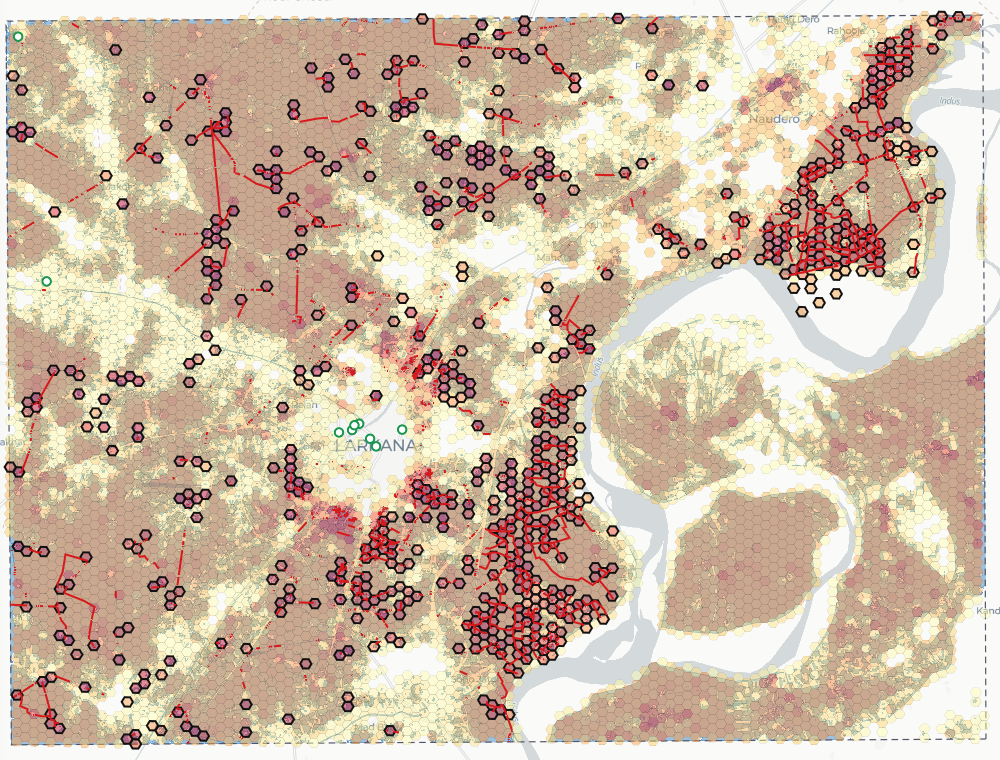
\includegraphics[width=\columnwidth]{figures/map_larkana.png}
\caption{Larkana, Sindh, 30 August 2022: priority per hexagon; dark outlines are cut-off hexagons, red lines roads under water. Buildings from OSM and ML footprints.}
\label{fig:larkana}
\end{figure}

\subsection{RQ5: Report trust under attack}\label{sec:trust}
Our rule: \emph{one report can send someone to look; it cannot send a boat, and neither can several that agree where the satellite has looked and seen no water.} A depth claim counts only when backed by satellite water in the hexagon or a neighbour or, only where the satellite has not mapped the hexagon at all, by two devices agreeing within one class. A depth read from the photo by the model needs the same backing (Sec.~\ref{sec:negative}). A people claim needs the model's count or two devices; satellite water confirms water, never people. Table~\ref{tab:threats} lists the main threats.

\begin{table}[t]
\caption{Threats and mitigations (full table in \texttt{THREAT\_MODEL.md}).}
\label{tab:threats}
\centering\scriptsize
\begin{tabular}{@{}p{22mm}p{58mm}@{}}
\toprule
Threat & Mitigation \\
\midrule
Stranger with the public key & The key alone writes nothing; only phones that redeemed a single-use invite insert, for their own team; teams, invites and devices unreadable \\
One person as many phones & One invite per phone, labelled by the issuing coordinator; the device id is the phone's server-signed identity, stamped by the database, so rate limits and corroboration count invites; revocation rejects past reports too \\
Reused or web photo & 64-bit difference hash against \trustRefs{} CVFD and European Flood 2013 images; $\le$\trustRejectBits{} bits rejected, 3--6 bits reviewed \\
Old photo & Capture time over 30 days old or in the future refused \\
One device inflating a hexagon & Each device counts once per hexagon; people are the maximum, not the sum \\
Gallery photo, spoofed GPS & EXIF first; device fix only if under 10\,min old; confidence from reported accuracy \\
Colluding devices & Device agreement never overrules a satellite map that says dry \\
\bottomrule
\end{tabular}
\end{table}

The hash catches \trustForwarded{} of \trustSample{} forwarded copies but only \trustCropped{} of 10\% centre crops; \trustBandShare{} of unrelated photos (\trustBandN{} of \trustEufloodN{}) fall in the review band, which is why only near-identical hashes are rejected outright. We injected synthetic reports into the Prague ranking, \atkDraws{} draws per scenario, assuming an attacker with a valid team code and photos that pass every check (Table~\ref{tab:attack}). Replaying the first version of the rule, which let two agreeing devices corroborate each other anywhere and let satellite water confirm people, put \permColludeInTop{} of 10 colluding pairs into the top ten (top-10 overlap \permColludeOverlap{}) and on average \permWetInTop{} lone reports inside mapped water there (overlap \permWetOverlap{}), none flagged. The current rule closes both. Its remaining weakness is the third row: inside water the satellite did map, a fabricated depth claim counts and moves the top ten a little. A leaked team code admits an outsider until it is retired.

\begin{table}[t]
\caption{Simulated attacks on the Prague ranking: top-10 overlap with the clean ranking and fake hexagons flagged for verification.}
\label{tab:attack}
\centering\scriptsize
\begin{tabular}{@{}p{38mm}rrrr@{}}
\toprule
 & \multicolumn{2}{c}{Current rule} & \multicolumn{2}{c}{First rule} \\
Scenario & Overlap & Flagged & Overlap & Flagged \\
\midrule
Lone reports, chest-deep, mapped-dry & \atkLoneOverlap{} & \atkLoneFlagged{} & \permLoneOverlap{} & \permLoneFlagged{} \\
Colluding device pairs, mapped-dry & \atkColludeOverlap{} & \atkColludeFlagged{} & \permColludeOverlap{} & \permColludeFlagged{} \\
Lone reports inside mapped water & \atkWetOverlap{} & \atkWetFlagged{} & \permWetOverlap{} & \permWetFlagged{} \\
\bottomrule
\end{tabular}
\end{table}

\subsection{Case study: what photos show}\label{sec:cases}
Of \eufLocated{} geotagged photos of the 2013 Central European floods~\cite{barz2018flood}, \agInAoi{} fall inside an EMS-mapped area; \agOwnHex{} have satellite water in their own hexagon and \agRing{} within one ring, and with permanent water counted the share is \agRingPerm{}, so a hexagon test cannot tell a high river from a flooded street. Distances can (Fig.~\ref{fig:dist}): in the Dresden area the median unique geotag is \agDresdenFlood{}\,m from mapped flood and \agDresdenRiver{}\,m from the river; in the Prague area it is \agPragueFlood{}\,m from mapped flood and \agPragueRiver{}\,m from the river, because the Vltava rose inside its embankments in the centre. On the Prague map of 3 June 2013, \pragueClosed{} roads are closed and \pragueCut{} hexagons cut off; the five highest-ranked hexagons are all cut off, in the southern districts at the Berounka confluence, while the \praguePhotos{} photos inside the mapped area cluster on the central embankments (Fig.~\ref{fig:map}). Photographers were not where the need was.

\begin{figure}[t]
\centering
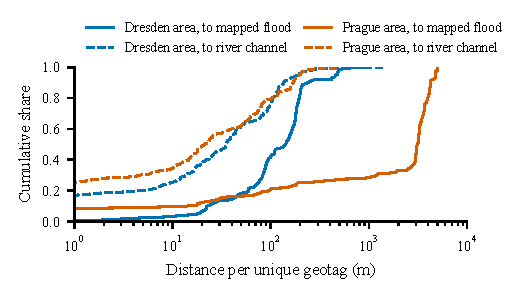
\includegraphics[width=\columnwidth]{figures/fig_distances.pdf}
\caption{Distances from geotagged 2013 photos to mapped flood (solid) and river channel (dashed), per unique geotag.}
\label{fig:dist}
\end{figure}

\begin{figure}[t]
\centering
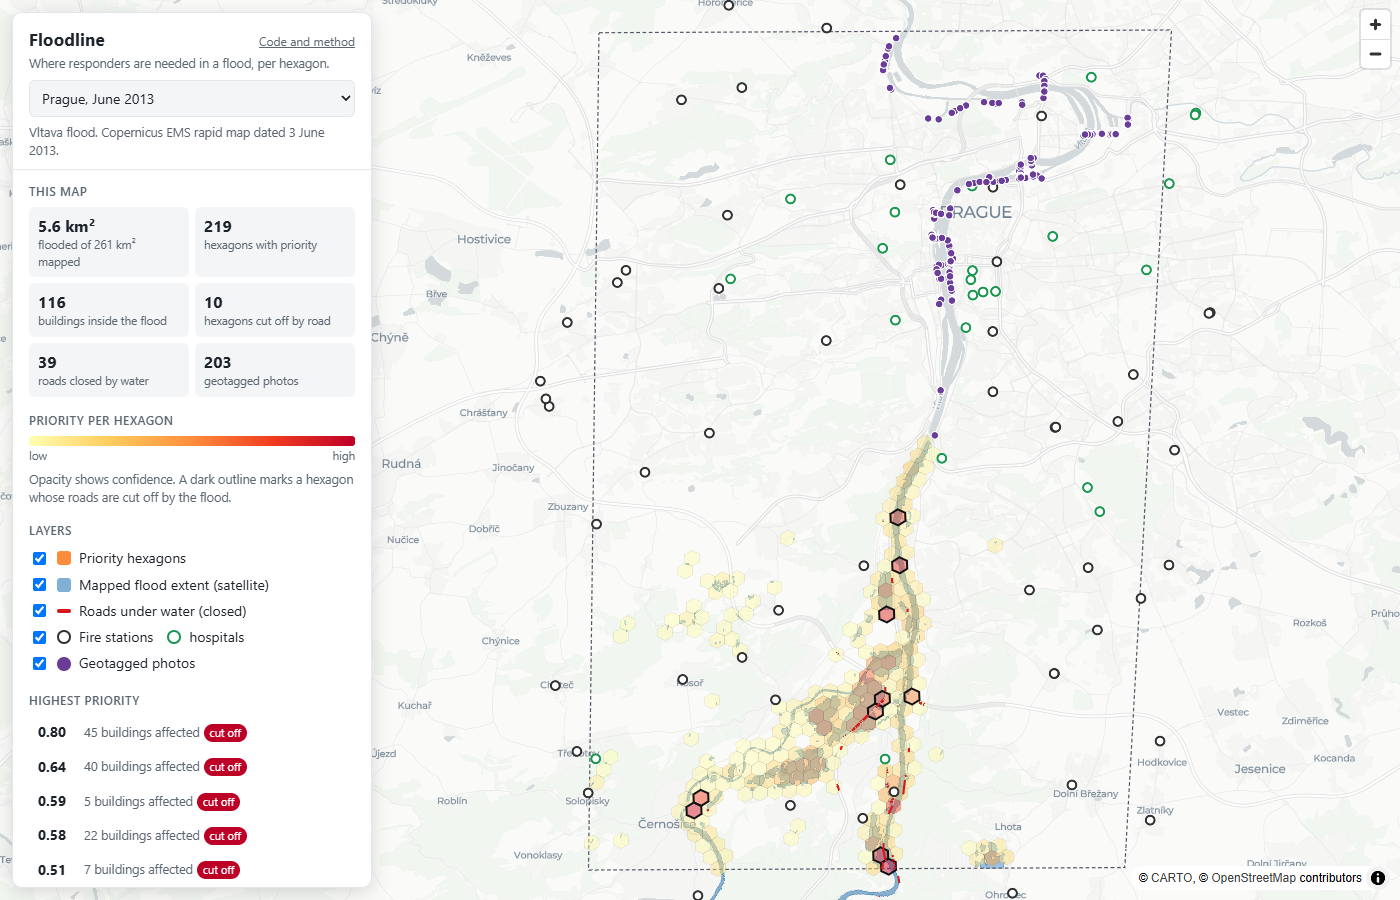
\includegraphics[width=\columnwidth]{figures/map_prague.png}
\caption{Prague, June 2013, in the web map: priority per hexagon, cut-off hexagons outlined, roads under water in red, photos in purple.}
\label{fig:map}
\end{figure}

\subsection{Negative results}\label{sec:negative}
\textbf{Depth from geometry.} Waterline geometry reads depth from how much of a person, car or door remains visible and accepts only water touching the object's base at its metric depth~\cite{yang2024depthv2}, on SAM~3 instance masks~\cite{carion2026sam3}. It gives an estimate for \wlWithEstimate{} of \wlImages{} images, \wlN{} of them in the depth benchmark, and there it is no better than always answering the commonest class (Table~\ref{tab:waterline}). Its errors are systematic: it recognises dry scenes (\wlDryRight{}) and calls ankle-deep water knee-deep (\wlAnkleKnee{}); the sample holds \wlAboveHeadN{} above-head images. The vision--language path~\cite{bai2025qwen3vl,llamacpp} fares no better on the \vlmN{} benchmark images it classifies: exact \vlmExact{} against \vlmBaseExact{} for the majority class, within one \vlmWithin{}. Its errors are one-sided: it calls most shallow water knee-deep but gets chest-deep and deeper water mostly right. We first let a model-read depth corroborate a report on its own; given these results it is now only a claim that needs satellite or second-device backing, and re-running the attack simulations after the change left every number unchanged. Segmentation itself is not the bottleneck: SAM~3 reaches a mean IoU of \samWaterMean{} for water (median \samWaterMedian{}, $n$=\samWaterN{}), \samPersonMean{} for people and \samBuildingMean{} for buildings on \samImages{} images, against masks that were themselves SAM~3-assisted, so partly circular.

\begin{table}[t]
\caption{Waterline depth class on the depth benchmark.}
\label{tab:waterline}
\centering\scriptsize
\begin{tabular}{@{}lrrrr@{}}
\toprule
Method & Exact & Within one & Mean error, bins & $n$ \\
\midrule
Waterline geometry & \wlExact{} & \wlWithin{} & \wlMAE{} & \wlN{} \\
Always ``ankle'' (majority) & \wlBaseExact{} & \wlBaseWithin{} & -- & \wlN{} \\
\bottomrule
\end{tabular}
\end{table}

\textbf{Fitted rules.} As RQ3 shows, choosing weights on five floods does not transfer to the sixth; we report the hand-set prior instead.

\textbf{Leakage in a public dataset.} Hashing for the trust model showed that the Close-View Flood Dataset (CVFD) contains \leakEuflood{} of the \trustEufloodN{} European Flood 2013 photos and that \leakTest{} of its \leakTestN{} test images have a near-copy in training. This does not affect Floodline, whose perception is zero-shot and trains on nothing, but it inflates any classifier trained and tested on CVFD; the dataset card now says so.

% ===============================================================================================================
\section{What a Coordinator Gets, and Reproducibility}

The map shows three layers: the ranked hexagons, the roads closed by water with the hexagons they cut off, and a verification list of report claims that nothing independent backs yet. The ranking answers ``where is damage likely''; the access layer answers ``can a ground team get there'' and is drawn even where it does not move the ranking, which is why RQ2's neutral result does not remove it. Confidence travels with each hexagon, so a high priority resting on one layer reads differently from one that three layers agree on.

Every stage writes a run manifest (code version, parameters, timing) next to its output, and this paper's numbers, tables and data figures are generated from those files by two scripts in the repository; a result that does not exist yet is printed as pending rather than estimated. OSM comes from dated extracts, the benchmark selection is a rule rather than a choice, and the field app's database rules are tested against Postgres in continuous integration.

% ===============================================================================================================
\section{Threats to Validity}

\textbf{Sample.} EMS grades towns where analysts were asked to look; they are not a random sample of flooded places, and \nTowns{} towns from six events give wide intervals. \textbf{Today's map.} Roads and buildings come from current OSM and ML footprints, not the map at the time of each flood, and closures ordered by authorities are not in the data. \textbf{Damage is a proxy for need.} Graded building damage misses cut-off but undamaged neighbourhoods by construction, which is exactly what access adds; RQ2 can show that access does not hurt damage capture, not that it helps responders. \textbf{One shared input.} The flood polygons used as hazard come from the same EMS products as the grading. \textbf{Depth labels.} The depth benchmark (\depthImages{} images, \depthUnknown{} unknown) was labelled from contact sheets with an AI assistant; a blind human review is pending. \textbf{No deployment.} The field app and trust model have been tested by simulation, not by responders in a live flood.

% ===============================================================================================================
\section{Conclusion}
Across six floods on four continents, a hand-set fusion of flood extent, buildings and road access puts \capEHA{} of graded damage into the top tenth of hexagons on average and, unlike the building, water, exposure and access layers on their own, does not collapse on any one flood. Fitting its weights makes it worse on floods it has not seen. It still depends on an analyst-quality flood map: radar alone does not yet rank towns well, and open building footprints matter most where OpenStreetMap is thin. Code, benchmark, map, field app and depth benchmark are open: \url{https://github.com/sunnyallana/floodline}, \url{https://floodline.sunnyshabanali.dev}, \url{https://huggingface.co/datasets/sunnyallana/flood-depth-benchmark}.

\section*{Acknowledgment}
Flood extent and grading \copyright{} European Union, Copernicus EMS; modified Copernicus Sentinel data via Microsoft Planetary Computer; map data \copyright{} OpenStreetMap contributors (ODbL); Microsoft Global ML Building Footprints; GHSL \copyright{} European Union; photos from Wikimedia Commons via the European Flood 2013 dataset, each under its own licence.

\bibliographystyle{IEEEtran}
\bibliography{references}

\end{document}
